\documentclass[12pt]{article}

\usepackage[utf8]{inputenc}%encodage des caractères
\usepackage{blindtext}
\usepackage[T1]{fontenc}%encodage de la police
\usepackage[french]{babel}%langue française
\usepackage{amsmath}
\usepackage{graphicx}
\usepackage[ruled,noline]{algorithm2e}
\usepackage{listings}
\usepackage{color}
\usepackage{float}
\usepackage{array}


\usepackage{url}
\usepackage{sectsty}
\usepackage{xcolor}

\usepackage{titling}%ajout de texte sur et sous le titre

%lien sans bordure
\usepackage[hypertexnames=false, pdftex]{hyperref}
\hypersetup{ colorlinks = true, linkcolor = black, urlcolor = red , citecolor = blue }

\definecolor{color_section}{RGB}{145,7,7}
\definecolor{color_subsection}{RGB}{120,40,40}
\definecolor{color_subsubsection}{RGB}{180, 40, 40}
\sectionfont{\color{color_section}\underline \small}
\subsectionfont{\color{color_subsection} \small}
\subsubsectionfont{\color{color_subsubsection}\small}

\usepackage{caption}
\captionsetup[figure]{font=small}

\title{\hrulefill \vspace{15pt} \\ \huge \textbf{Jeu d'assemblage de formes} \\ \vspace{20pt} \hrulefill  \small \textit{Méthode de conception logiciel\hrulefill \vspace{40pt}}}

\author{ Marguerite Bauchez 21803320 \and Olivier Cocquerez 21803239  \and Paul Lebranchu 21403460 \and Raphaelle Lemaire 21802756  }

\date{}	
\input{insbox}

\begin{document}
	
	
	
\begin{titlepage}

     \renewcommand{\maketitlehooka}{
     

     \begin{flushright} \today \end{flushright}
     
     
\includegraphics[scale=1]{Images/logo.png}
     
     \vspace{65pt}}
	
	
	\renewcommand{\maketitlehookd}{
	\vspace{65pt}
		
	\begin{flushright} L3 informatique \\ Groupe 1B \\ 2020-2021
	\end{flushright}
	}
     
	\maketitle
	
	\setcounter{page}{0}
\end{titlepage}


\newpage
\tableofcontents
\setcounter{page}{0}
\newpage

\section*{Introduction}


\begin{small}
	Le jeu d'assemblage de formes est un jeu de puzzle où l'on doit constituer une forme à l'aide de différentes pièces de forme et de taille aléatoire de façon à ce que la forme puisse rentrer dans un rectangle dont la taille devra être la plus petite possible.
Afin de réaliser ce jeu, nous avons utilisé le langage de programmation objet Java et fait un dépôt sur SVN pour pouvoir travailler en équipe (même à distance). Ce jeu sera aussi jouable dans le terminale de commande.

\end{small}

\section{Organisation du projet}

\subsection{Organisation des fichiers}

Lorsque nous récupérons le projet depuis svn, les répertoires sont organisés de la façon suivante:

\begin{small}
\begin{itemize}
	\item un répertoire livraison contenant:
	\begin{itemize}
		\item un répertoire dist contenant toute les ressources nécessaire au lancement de l'application (.jar + contenu du répertoire lib)
		\item un répertoire doc qui contiendra la javadoc des classes présentes dans le répertoire src
		\item un répertoire lib qui contient les images du jeu ainsi qu'une archive .jar permettant de générer les pièces de jeu
		\item un répertoire rapport qui contient ce rapport au format pdf ainsi qu'un répertoire LaTeX contenant l'ensemble des ressources nécessaire à la création de ce pdf
		\item un répertoire src qui contient l'ensemble des classes nécessaires pour faire tourner le jeu d'assemblage, ce répertoire est divisé de la façon suivante:
		\begin{itemize}
			\item un répertoire Controlleur qui contient les interfaces/classes abstraites nécessaires pour que la Vue et le Modele communiquent
			\item un répertoire Modele qui contient les classes permettant de générer un Plateau de jeu et les méthodes nécessaires pour agir sur ce plateau
			\item un répertoire Vue qui contient les classes nécessaire pour donner un aspect visuel et interactif au Modele
			\item un fichier Main.java qui permet de lancer l'application 
		\end{itemize}
		\item un ficher build.xml qui permet de compiler le code, qui créé un répertoire build contenant tout les fichier .class, qui génère la javadoc des classes présentes dans src et les stock dans le répertoire doc, qui recréer le contenu du répertoire dist et qui lance le jeu.
		\item un fichier README.txt qui explique à l'utilisateur comment lancer l'application et qui lui explique les deux modes de jeu disponible.
		\item un fichier score.txt vide qui contiendra les scores des différentes parties jouées. 
	\end{itemize}
	\item un répertoire piecesPuzzle contenant tout les classes qui se rapportent au pièce de jeu et un fichier ant qui génère la javadoc et une archive .jar qui sera placé automatiquement dans le répertoire lib de livraison.
\end{itemize}
\end{small}

\subsection{Gestion du projet}

Pour gérer ce projet, nous avons fait appel à plusieurs ressources: 
\begin{small}
\begin{itemize}
	\item SVN pour mettre en commun nos fichiers 
	\item Discord/messenger pour pouvoir communiquer entre nous et nous tenir au courant des différentes avancées effectuées
	\item Les cours (e-campus/discord/cours en présentiels) 
	\item Atom/NetBeans/Geany pour rédiger notre code
	\item Oracle (https://docs.oracle.com/javase/8/docs/api/)
	\item Trello pour nous répartir le travail
\end{itemize}
\end{small}
\section{Architecture du projet}

\subsection{Diagramme de la librairie piece}

La librairie pieces nous permet de construire les différentes pièces de jeu. Elle utilise le design pattern strategy: elle est composée d'une interface (InterfacePiece) qui nous donne les propriétés à implémenter pour les différentes pièces (rotation et déplacement), une classe abstraite qui définit les spécificités des pièces de notre jeu en particulier: cette classe défini les paramètres des pièces:leur position x et y, leur taille minimale et maximale, leur largeur, leur hauteur, le tableau définissant la pièce (rempli avec des 1 et des 0) et leur identifiant. C'est cette classe qui définit la rotation des pièces(rotation du tableau définissant la pièce) et leur déplacement: la fonction prend en paramètre un entier x et un entier y qui seront les nouvelles coordonnées de la pièce. Ensuite, chaque sous-classe définit les spécificités de sa pièce (par exemple, pour une pièce de type O, la largeur et la hauteur doivent être identique) et créé la pièce en utilisant sa version du createPiece().Nous trouvons également dans ce package une classe PieceFactory (pattern Factory) qui nous permet de créer des instances d'un objet en fonction du type qu'on lui a attribué en paramètre.


\begin{figure}[h]
\begin{center}
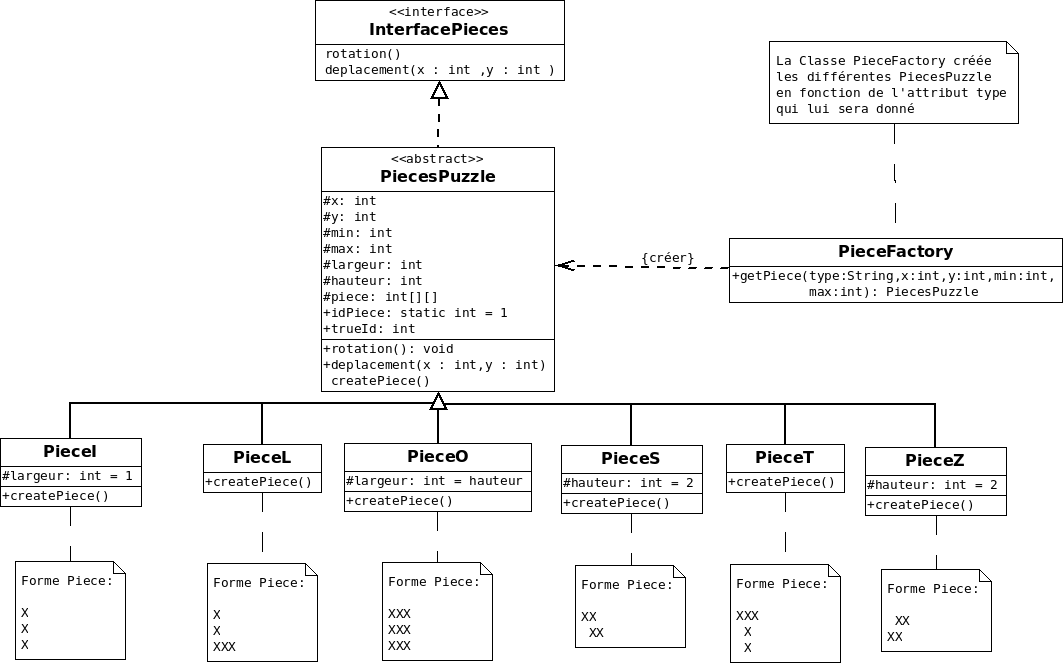
\includegraphics[scale=0.22]{Images/libPiece.png}
\end{center}
\caption{Diagramme de classe: librairie pieces}
\end{figure}

\subsection{Diagramme de livraison}

Sur le diagramme ci-dessous, nous pouvons les interactions entre les différents packages qui composent notre projet. Nous constatons qu'il y a trois gros packages: le package Controlleur qui permet de faire le lien entre la vue et le modèle, le package Model qui gère la création du plateau et les méthodes pour interagir dessus et le package Vue qui gère l'interface graphique et les actions sur cette dernière.

Nous pouvons noter que trois classes ont recours à la librairie pieces :  la classe CreationPlateau (Model) et les classe Menu et AffPlateau (Vue).

Nous voyons que le package Model est constitué de trois classes: Plateau qui s’occupe des paramètres du plateau de jeu (taille), CreationPlateau qui appelle Plateau et qui étend la classe AbstractModeleEcoutable pour faire en sorte que la vue puisse écouter le modèle et la classe Main qui est là pour rendre le jeu jouable en version console.

Le package Vue est composé de quatre classes: une classe AffPlateau qui créera et affichera le plateau de jeu, une classe Menu qui gère le menu est les contrôles des pièces, cette classe possède une instance de CreationPlateau et une instance d'AffPlateau et fais le lien entre les deux grâce à sa méthode modeleMiseAJour (héritée de l'interface EcouteurModel). La classe Fenêtre est un JPanel qui prend en paramètre un objet de type Menu et qui l'affiche. Cette Fenetre est ensuite placée dans une JFrame dans la classe Affichage (classe permettant de lancé le jeu en mode interface graphique).

La classe Main appelle une instance de Modele.Main et une instance d'Affichage pour faire en sorte que le jeu soit jouable en mode console ou en mode interface graphique.

\begin{figure}[h]
\begin{center}
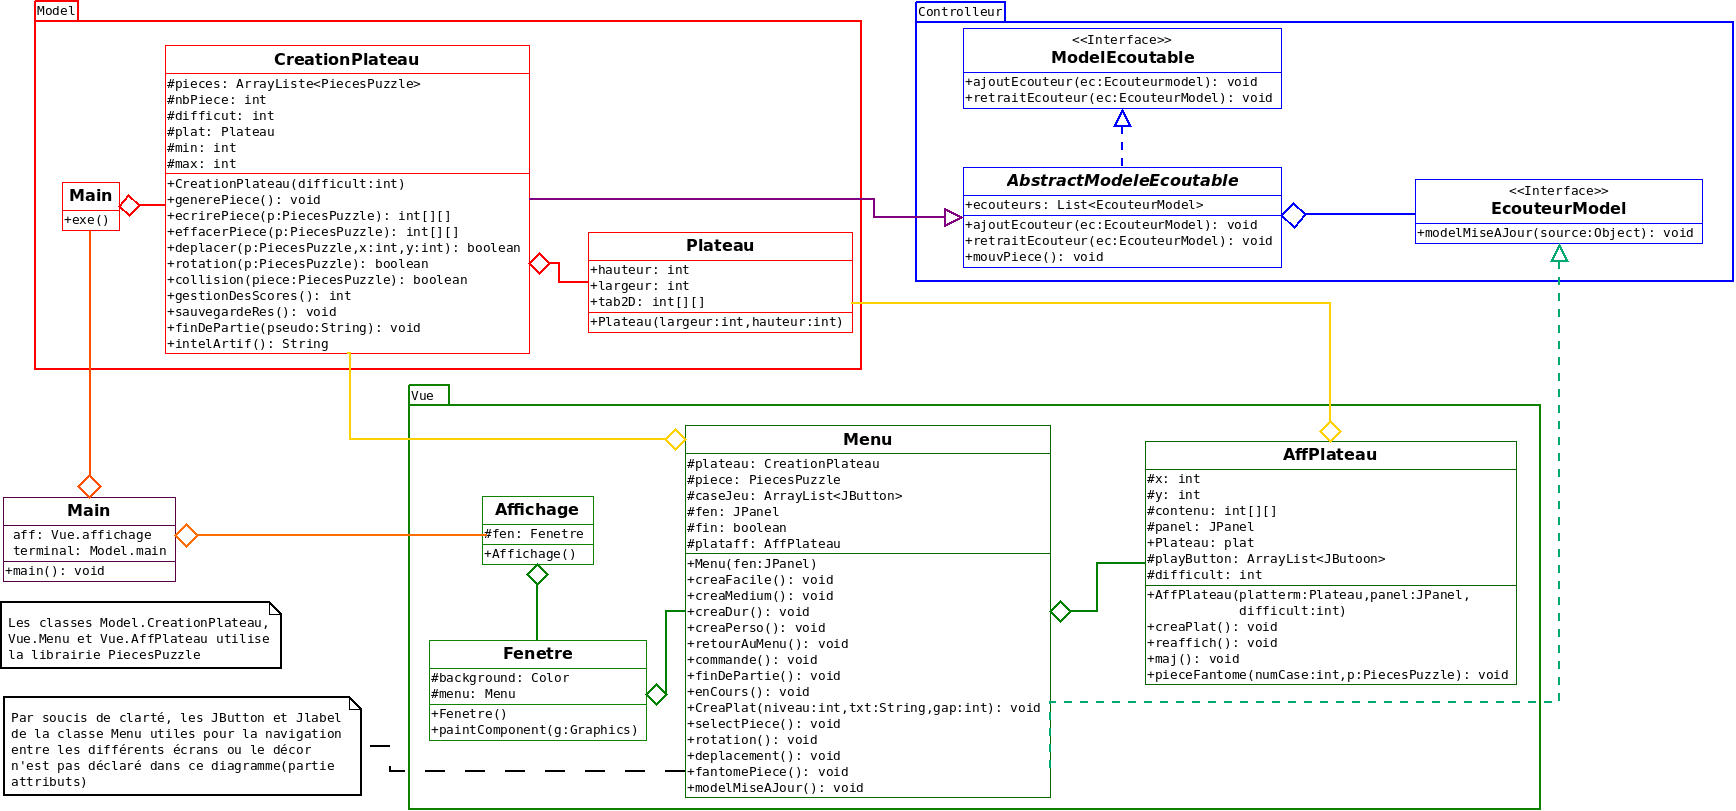
\includegraphics[scale=0.25]{Images/DiagClasse.png}
\end{center}
\caption{Diagramme de classe: répertoire src dans livraison}
\end{figure}

\section{Cas d'utilisation}

\InsertBoxR{0}{\quad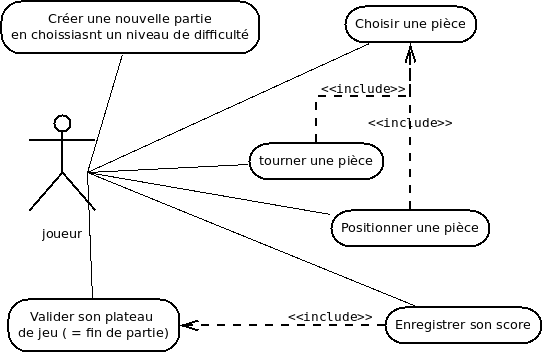
\includegraphics[scale=0.3]{Images/utilisateur.png}\quad}

L'utilisateur aura plusieurs actions à faire. Dans un premier temps, il devra créer une partie: Pour cela, il devra choisir son niveau de difficulté (cliqué sur un bouton dans le mode interface graphique, rentrer un int dans le mode console). Une fois le plateau de jeu créé, le joueur devra sélectionner une pièce et effectuer une action (rotation ou déplacement), dans le mode graphique cela se fait avec le clavier et la souris et dans le mode console, le joueur devra rentrer des commandes dans le terminal. Quand l'utilisateur estimera qu'il ne pourra pas faire mieux, il terminera la partie et aura la possibilité d'enregistrer son score. Une fois que cela sera fait, le joueur verra son score et celui de l'IA qu'il aura affronté et pourra commencer une nouvelle partie.

\subsection{Mode Console}


Dans un premier temps, on présente les différents niveaux de difficulté au joueur et on lui demande de sélectionner le niveau de son choix, une fois le niveau choisis, on montre la création du plateau pièce par pièce au joueur puis le joueur aura la possibilité de jouer. Lorsque l'utilisateur aura fini de jouer, on lui demandera de rentrer son pseudo pour la sauvegarde des scores, on affiche ensuite son score puis l'IA fait son calcul et nous affiche le sien, on demande ensuite à l'utilisateur s'il souhaite rejouer ou s'arrêter là, s'il rejoue, nous retournons à la création de partie, sinon le programme s'arrête.
\begin{figure}[h]
\begin{center}
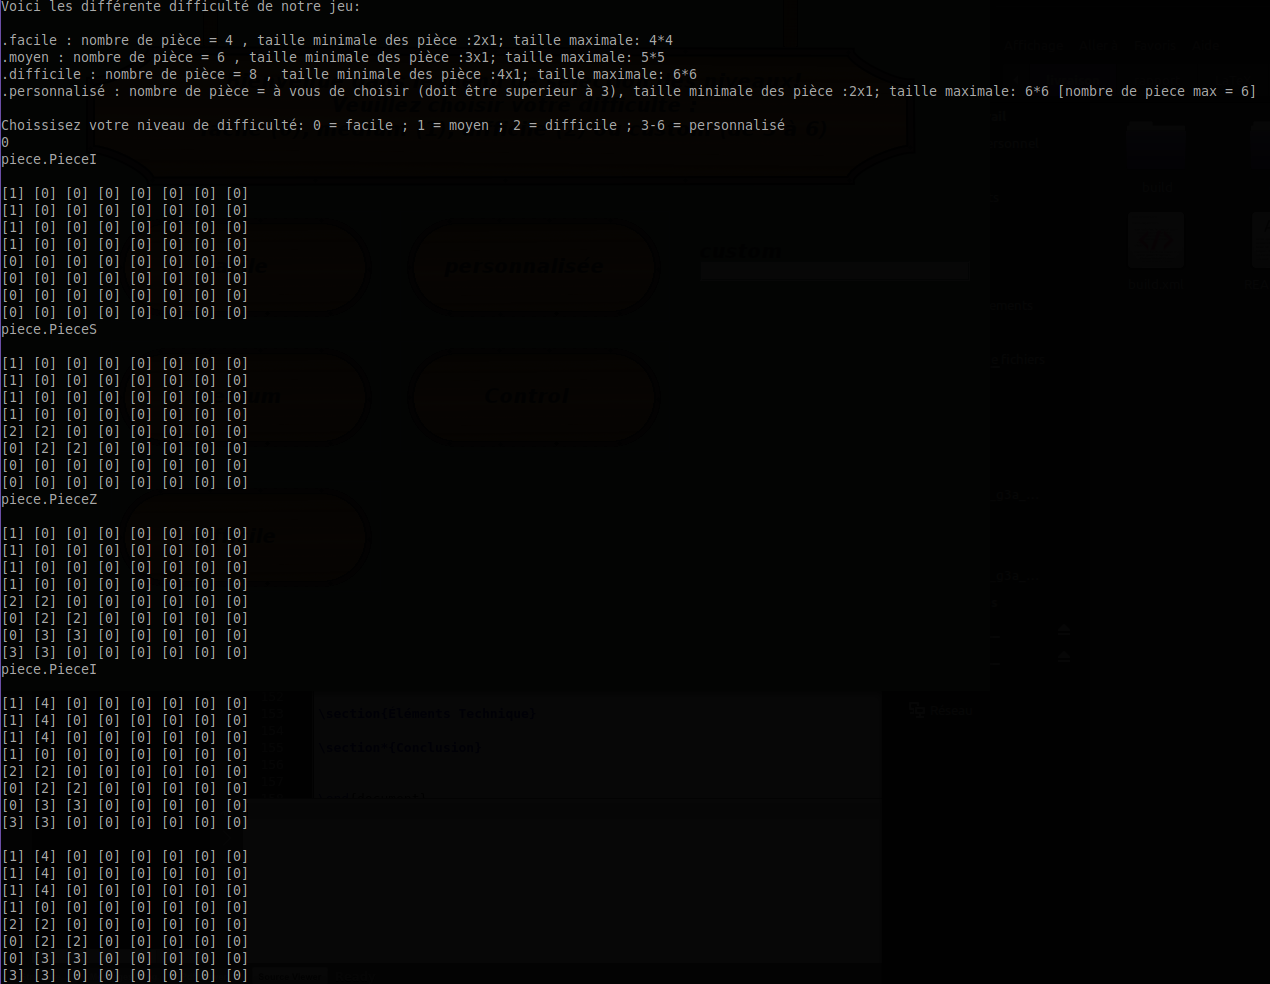
\includegraphics[scale=0.15]{Images/creationPartieCons.png}
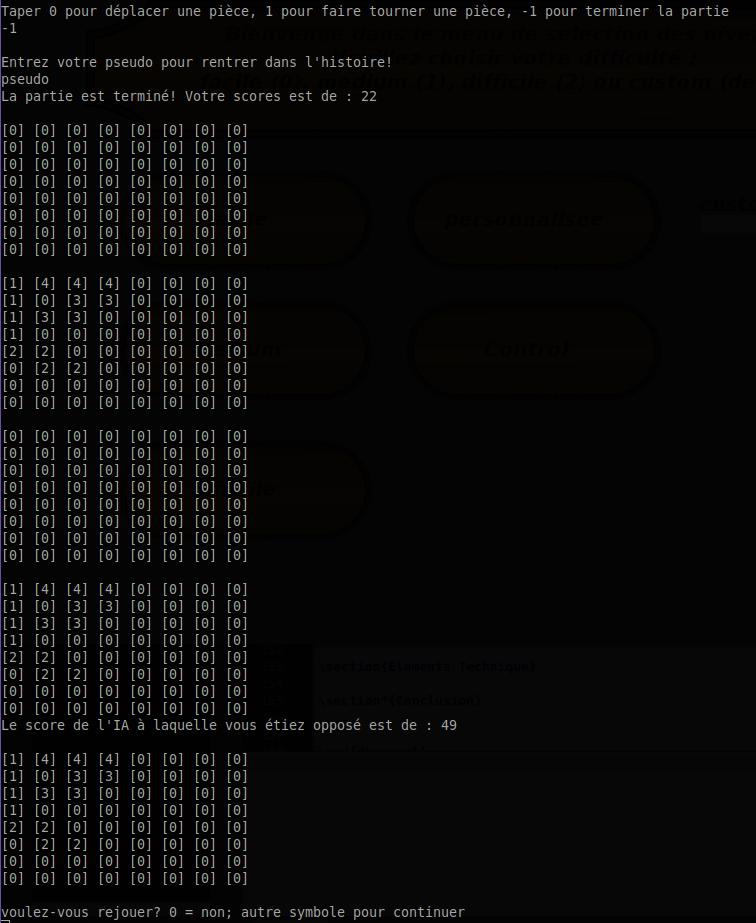
\includegraphics[scale=0.16]{Images/finPartieCons.png}
\end{center}
\caption{Début et fin de partie en mode console}
\end{figure}


Nous pouvons voir sur ces images de la figure 4 le déroulement des différent actions de jeu. Dans un premier temps, nous devons dire si nous souhaitons effectué une rotation ou un déplacement, si nous effectuons une rotation, nous avons juste à renseigner la pièce que nous souhaitons faire tourner, vous pouvez voir sur l'image de gauche une rotation réussie(cadre vert) et une rotation qui a échoué à cause d'une collision(cadre rouge).Si l'on souhaite effectuer un déplacement, nous devrons en plus renseigner un numéro de ligne et de colonne, vous pouvez voir dans le cadre vert un exemple de déplacement réussi et dans le cadre rouge, un exemple de déplacement raté. Le cadre jaune dans l'image de gauche nous montre que tant qu'on aura pas saisie un numéro de pièce valide pour une action, le programme nous redemandera de saisir un numéro de pièce.

\begin{figure}[h]
\begin{center}
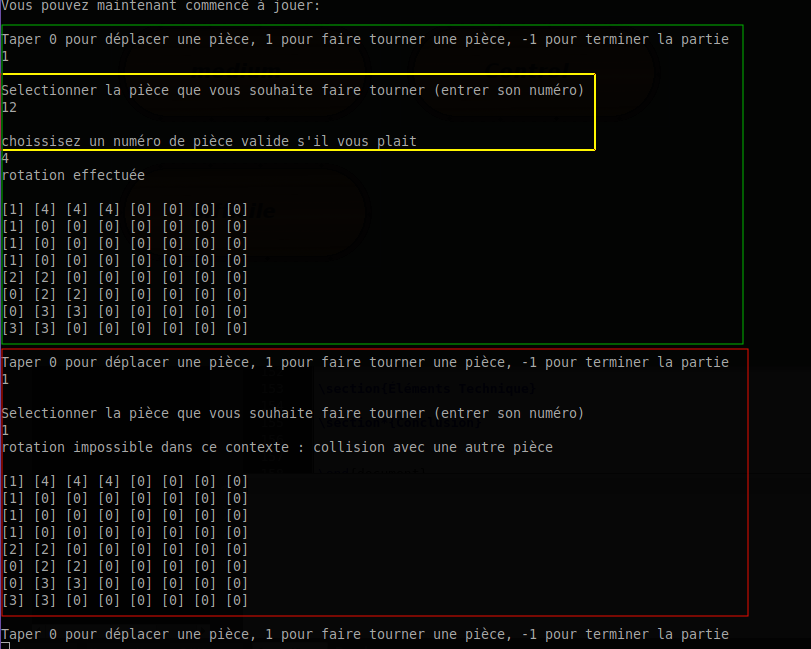
\includegraphics[scale=0.198]{Images/Rotation.png}
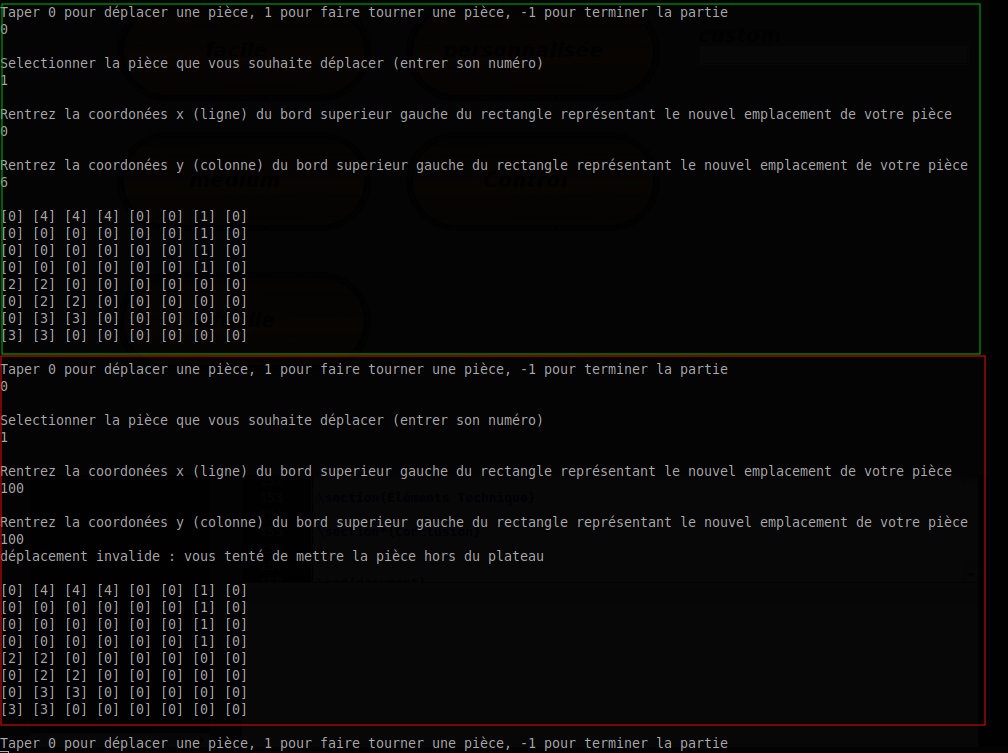
\includegraphics[scale=0.17]{Images/Deplacement.png}
\end{center}
\caption{jeu en mode console}
\end{figure}

\subsection{Mode Interface Graphique}
La figure 5 représente les différentes versions du menu qui existe, la première version correspond à ce qui s'affiche lorsqu'on lance l'application, la deuxième nous montre le menu lorsque nous tentons de créer une partie personnalisée en ne donnant pas les bonnes informations et la troisième version nous montre le menu lorsque nous retournons sur le menu lors d'une partie en cours.

\begin{figure}[h]
\begin{center}
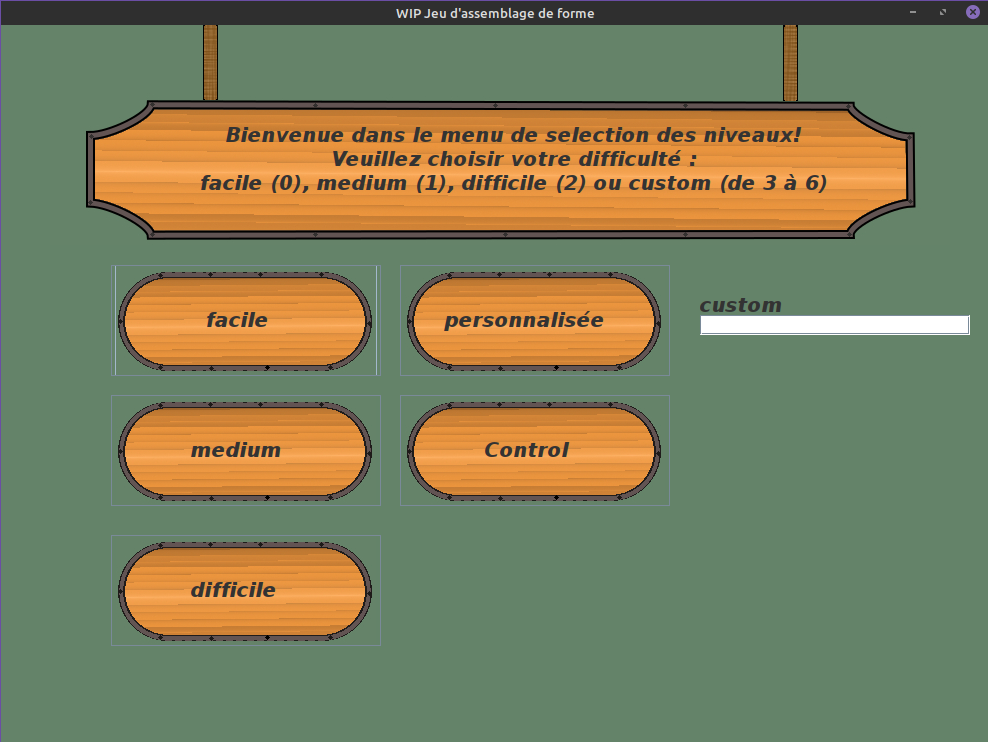
\includegraphics[scale=0.125]{Images/Menu1.png}
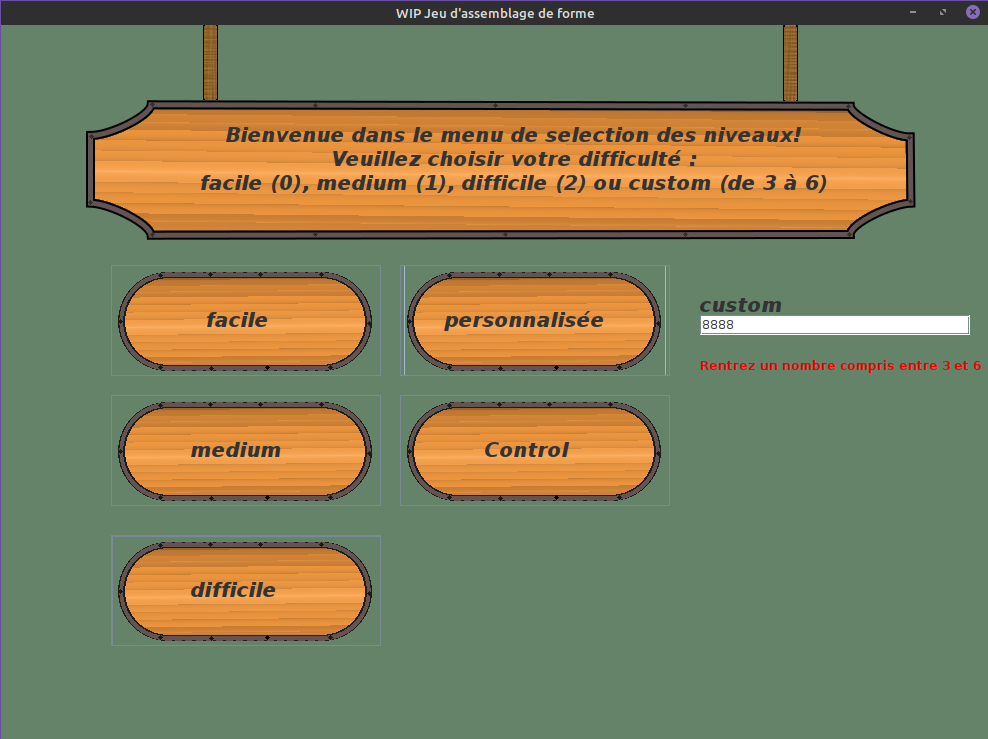
\includegraphics[scale=0.125]{Images/menu2.png}
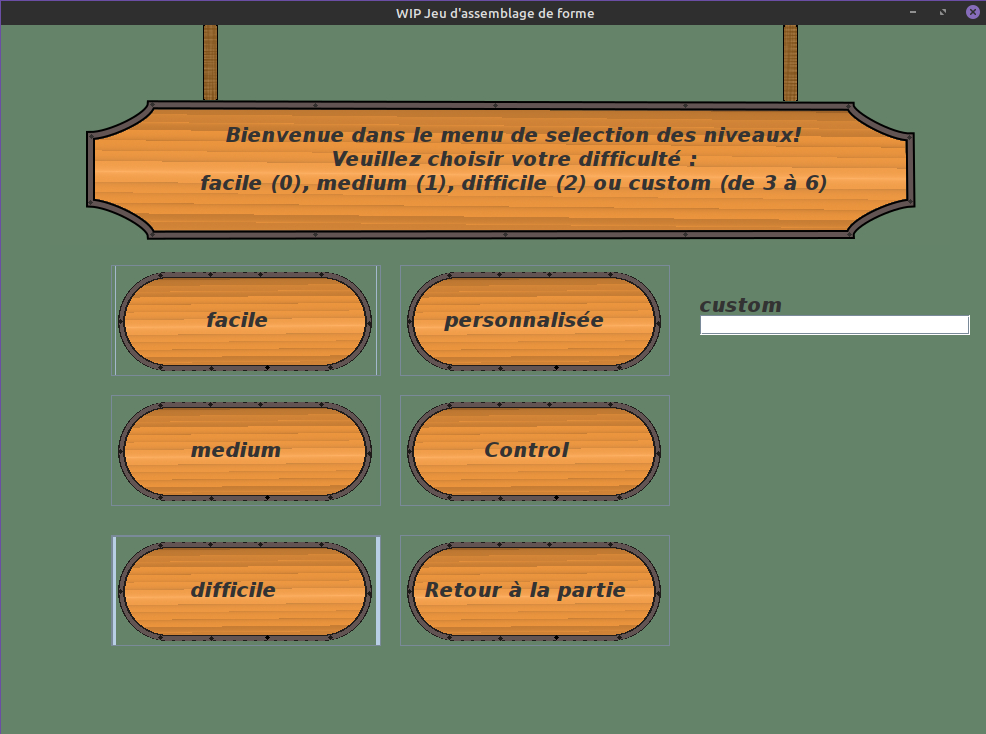
\includegraphics[scale=0.125]{Images/Menu3.png}
\end{center}
\caption{Les trois versions du menu}
\end{figure}

La figure 6 nous montre une partie en cours, la première image représente le plateau de jeu tel qu'il est créé, la seconde image nous montre une pièce fantôme de la pièce jaune qui est la pièce sélectionnée et les deux dernières images correspondent au fenêtre qui s'ouvre lorsque nous commettons une erreur lors du déplacement ou de la rotation d'une pièce.


\begin{figure}[h]
\begin{center}
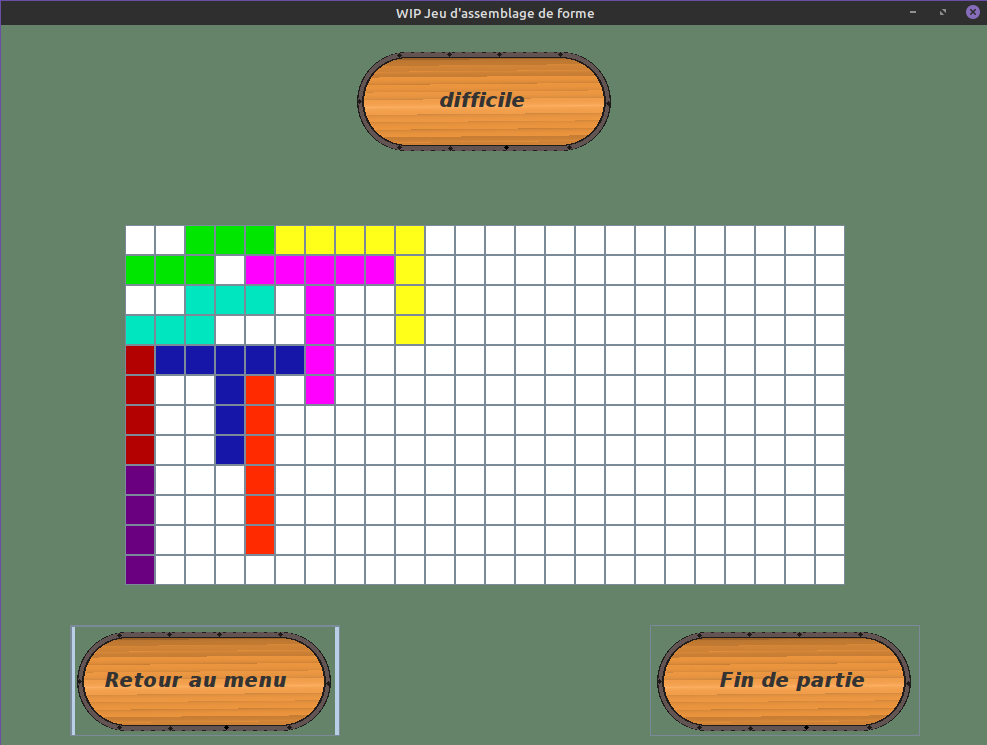
\includegraphics[scale=0.125]{Images/Jeu1.png}
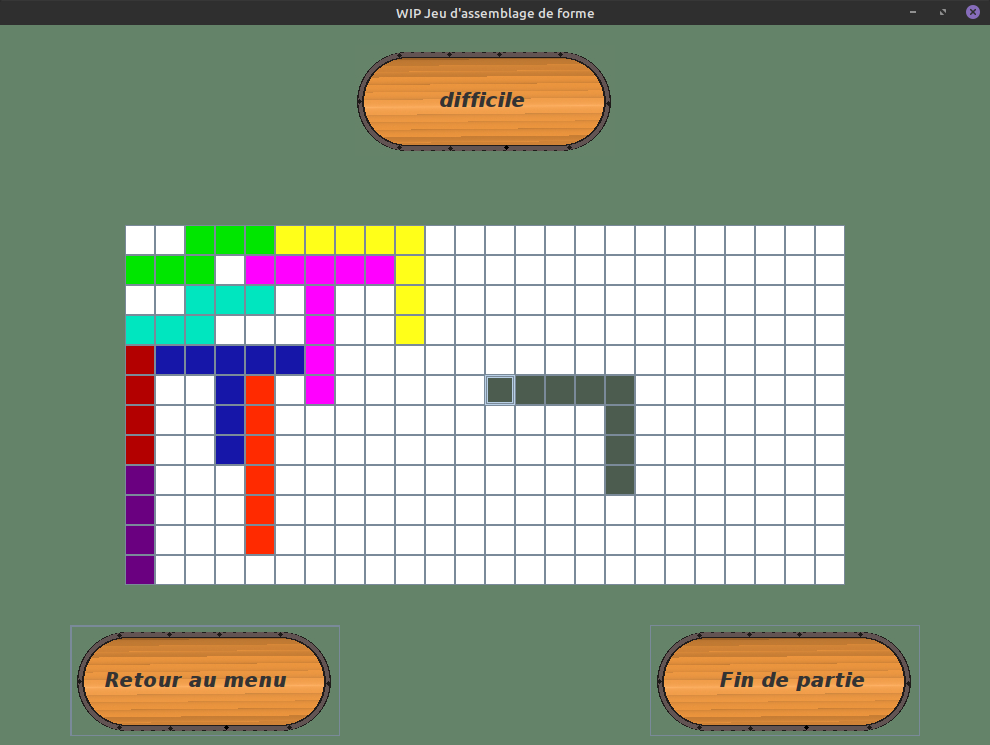
\includegraphics[scale=0.125]{Images/Jeu2.png}
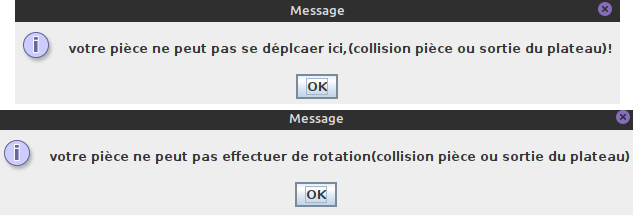
\includegraphics[scale=0.2]{Images/erreur.png}
\end{center}
\caption{Jeu}
\end{figure}

\vspace{20pt}
La figure 7 nous montre comment se déroule une fin de partie, dans un premier temps, nous appuyons sur le bouton fin de partie puis nous voyons une fenêtre apparaître et nous demander de rentrer notre pseudo. Ensuite, on voit apparaître notre score ainsi que le score de l'IA. Puis nous pouvons retourner au menu et créer une nouvelle partie. La dernière image nous montre le panneau affichant les controls du jeu, cette écran est accessible depuis le menu.

\begin{figure}[h]
\begin{center}
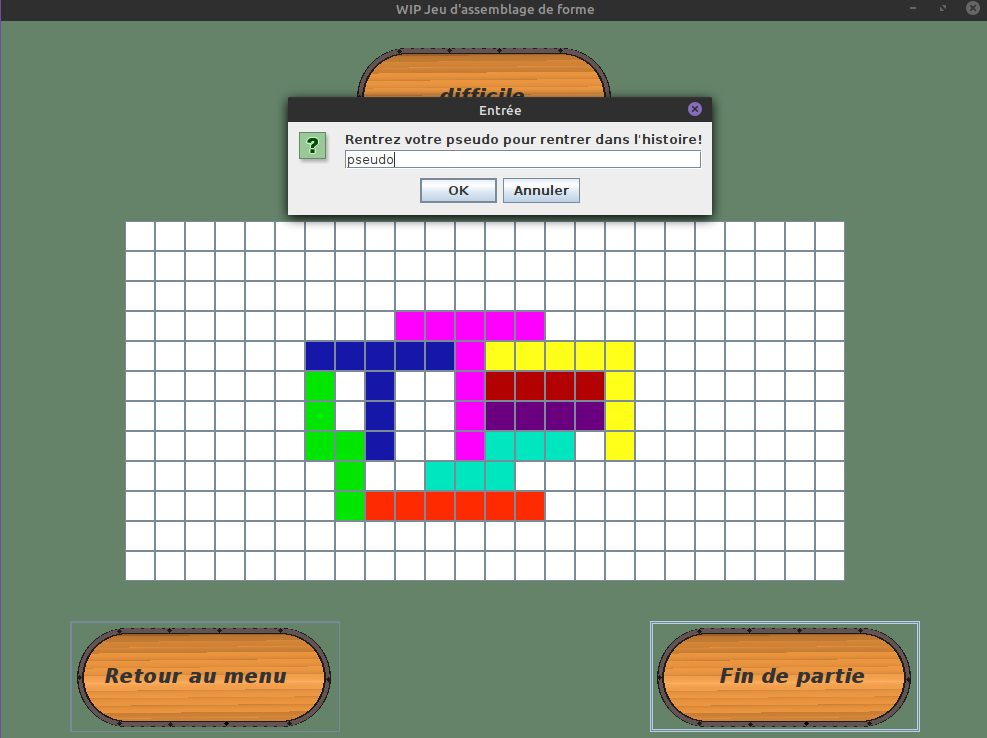
\includegraphics[scale=0.125]{Images/fin1.png}
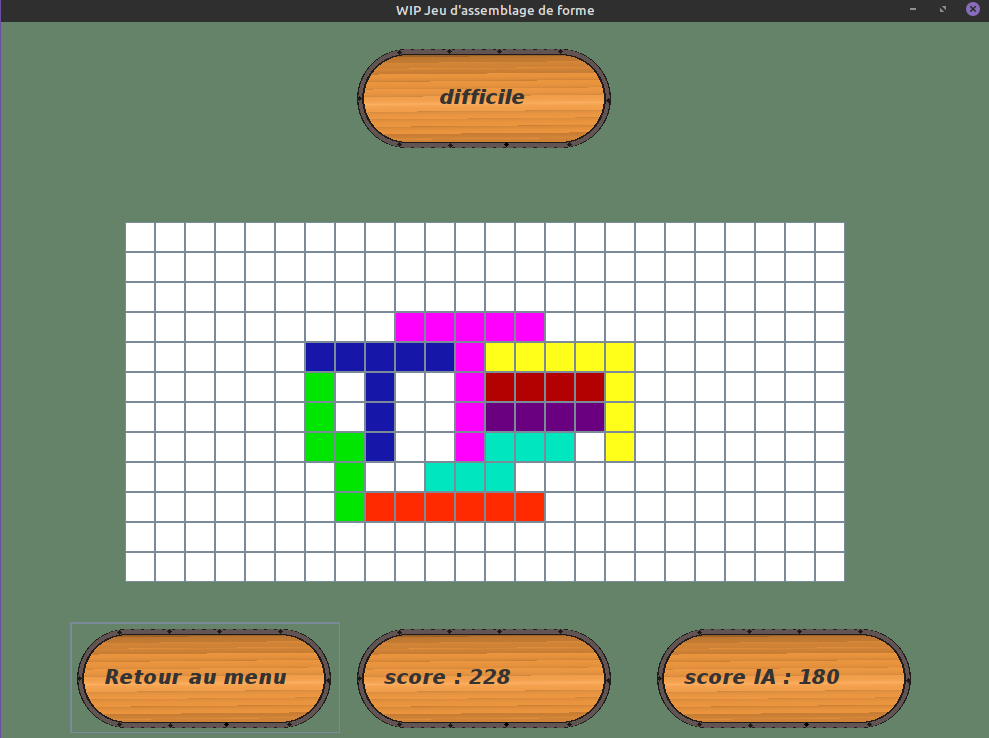
\includegraphics[scale=0.125]{Images/fin2.png}
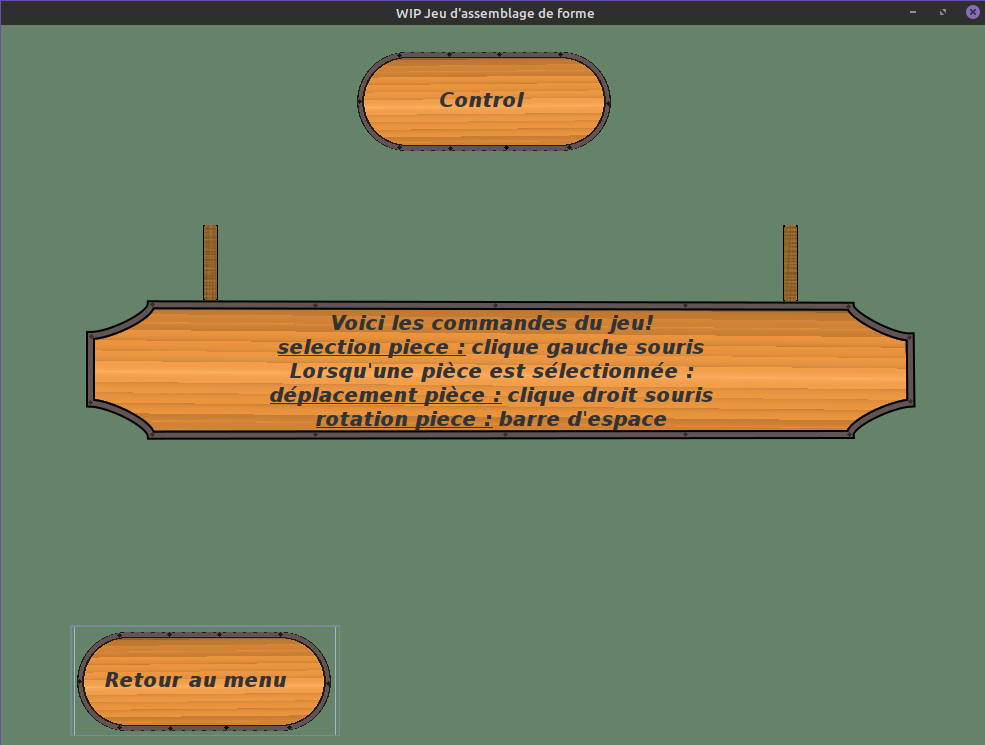
\includegraphics[scale=0.125]{Images/Control.png}
\end{center}
\caption{fin de partie et contrôles}

\end{figure}


\section*{Conclusion}
\begin{small}
Notre application est donc jouable en mode console comme en mode interface graphique.Cependant, quelques points de notre application pourraient être améliorer: notre IA se retrouve parfois bloquer dans des boucles infinies et nous renvoie une erreur, nous pourrions également ajouter des ascenseurs verticaux et horizontaux sur notre jeu pour les utilisateurs qui voudraient réduire la taille de leur fenêtre en mode  interface graphique.
\end{small}
\end{document}